\documentclass[11pt,a4paper]{article}
\usepackage{amsmath}\usepackage{amssymb}\usepackage[table]{xcolor}
\usepackage{tabularx}\usepackage{multirow}\usepackage{geometry}
\usepackage{enumitem}\usepackage{parskip}\usepackage{titlesec}
\usepackage{tocloft}\usepackage[most]{tcolorbox}
\usepackage{tikz}\usepackage{pgfplots}\pgfplotsset{compat=1.18}\usetikzlibrary{arrows.meta,calc,positioning,shapes.geometric,patterns}
\geometry{margin=2.5cm}
\titleformat{\section}{\large\bfseries}{}{0em}{}
\setlength{\cftbeforesecskip}{6pt}
\definecolor{q1color}{HTML}{D6EAF8}\definecolor{q2color}{HTML}{D5F5E3}
\definecolor{q3color}{HTML}{FDEBD0}\definecolor{q4color}{HTML}{F9E79F}
\definecolor{q5color}{HTML}{E8DAEF}\definecolor{q6color}{HTML}{FADBD8}
\definecolor{q7color}{HTML}{D1F2EB}\definecolor{q8color}{HTML}{FCF3CF}
\definecolor{q9color}{HTML}{EBDEF0}\definecolor{q10color}{HTML}{F5EEF8}
\newenvironment{mstab}[1]{%
  {\color{#1!75!black}\nobreak Mark Scheme}\par\nopagebreak\smallskip
  \arrayrulecolor{#1!70!black}\renewcommand{\arraystretch}{1.3}%
  \tabularx{\textwidth}{|>{\columncolor{#1!12}\raggedright\arraybackslash}p{1.9cm}|>{\columncolor{#1!12}}X|>{\columncolor{#1!12}\centering\arraybackslash}p{1.1cm}|}%
  \hline\rowcolor{#1!45} Question & Answer & Marks \\ \hline}{%
  \endtabularx\arrayrulecolor{black}\par\medskip}
\newtcolorbox{ansbox}[1]{colback=#1!8,colbacktitle=#1!30,colframe=#1!70!black,coltitle=black,fonttitle=\normalfont,title=Worked Solution,boxrule=0.6pt,arc=2mm,left=4pt,right=4pt,top=4pt,bottom=4pt,breakable}
\newcommand{\topiclabel}[1]{\hfill\normalfont\small\itshape\textcolor{black!55}{#1}}
\newcommand{\examq}[4]{\section[#1 - Q#2]{#1 - Q#2 - #3 - #4}}
\begin{document}
\begin{center}
  {\LARGE \textbf{Cambridge O Level Physics 5054/21/M/J/16}}\\[6pt]
  {\large May/June 2016 -- Mark Scheme \& Worked Solutions}
\end{center}
\bigskip

%=================================================================
\examq{5054/21/M/J/16}{1}{Forces or Dynamics \textperiodcentered\ Motion or Kinematics}{5}

\begin{mstab}{q1color}
 & air resistance is zero\newline or no air resistance acts (at first)\newline or weight much larger than air resistance & B1 \\ \cline{2-3}
\multirow{-2}{1.9cm}{1(a)} & $(a =)\ F/m$ or weight\,/\,mass or $600/60$\newline or weight is 10 times mass & B1 \\ \hline
1(b) & air resistance\,/\,upwards force is larger than weight\,/\,600\,N\,/\,downwards force & B1 \\ \hline
1(c)(i) & $5(.0)$\,m\,/\,s & B1 \\ \hline
1(c)(ii) & 120\,N & B1 \\ \hline
\end{mstab}

\begin{ansbox}{q1color}
For (a), the acceleration is set by the \emph{resultant} force through Newton's second law, $F = ma$. At the instant the sky-diver leaves the balloon he is stationary, and air resistance depends on speed, so at zero speed the air resistance is \textbf{zero} (or at least negligible beside his weight). The only force acting is therefore his weight, $600$\,N downwards, and
\[ a = \frac{F}{m} = \frac{\text{weight}}{\text{mass}} = \frac{600}{60} = 10\ \mathrm{m/s^2}\ \text{(downwards)}. \]
Equivalently, his weight in newtons is 10 times his mass in kilograms, so the initial acceleration is numerically $10\,\mathrm{m/s^2}$ -- the acceleration of free fall.

For (b), opening the parachute hugely increases the area presented to the air, so the air resistance jumps to a value \textbf{larger than the weight} of $600$\,N. The resultant force is now $(\text{air resistance} - 600)$ newtons acting \emph{upwards}, and since acceleration is in the direction of the resultant force, the acceleration is upwards. (He is still moving downwards -- he is slowing down.)

For (c)(i), at terminal velocity the acceleration is zero, so the forces balance: the air resistance must equal the weight of $600$\,N. Reading Fig.\,1.2 across from $600$\,N on the air-resistance axis to the curve, and then down to the speed axis, gives
\[ \text{terminal velocity} = 5.0\ \mathrm{m\,/\,s}. \]

For (c)(ii), read the air resistance at $5.5$\,m\,/\,s from Fig.\,1.2; the curve gives $720$\,N. The weight is $600$\,N downwards, so
\[ \text{resultant} = 720 - 600 = 120\ \mathrm{N}\ \text{(upwards)}. \]
The sign makes sense: he is above terminal velocity, so the net force decelerates him back towards $5.0$\,m\,/\,s.
\end{ansbox}

%=================================================================
\examq{5054/21/M/J/16}{2}{Deformation \textperiodcentered\ Mass Weight and Density}{5}

\begin{mstab}{q2color}
2(a)(i) & limit of proportionality & B1 \\ \hline
2(a)(ii) & 250\,g & B1 \\ \hline
2(a)(iii) & 2.5\,N & B1 \\ \hline
 & half the extension\,/\,10\,cm & B1 \\ \cline{2-3}
\multirow{-2}{1.9cm}{2(b)} & each\,/\,both\,/\,another spring shares\,/\,distributes the weight\,/\,mass\newline or both springs bear\,/\,carry the load & B1 \\ \hline
\end{mstab}

\begin{ansbox}{q2color}
For (a)(i), up to point P the graph is a straight line through the origin, so extension is directly proportional to the load. P is where that proportionality breaks down, so it is the \textbf{limit of proportionality}. (Hooke's law applies only below P.)

For (a)(ii), read the extension from Fig.\,2.1 first. The unloaded spring is $10$\,cm long and with X attached it is $30$\,cm long, so
\[ \text{extension} = 30 - 10 = 20\ \mathrm{cm}. \]
Going across Fig.\,2.2 at an extension of $20$\,cm and down to the mass axis gives
\[ \text{mass X} = 250\ \mathrm{g}. \]
(Note that $20$\,cm is still on the straight part of the graph, below P, so the reading is reliable.)

For (a)(iii), convert to kilograms and use $W = mg$:
\[ W = mg = 0.250 \times 10 = 2.5\ \mathrm{N}. \]

For (b), in Fig.\,2.3 the same mass X hangs from \emph{two} identical springs side by side, so the two springs \textbf{share the load}: each one now carries only half the weight, $1.25$\,N instead of $2.5$\,N. Each spring is still obeying Hooke's law ($\text{extension} \propto \text{load}$), so halving the load on a spring halves its extension. The extension is therefore
\[ \tfrac{1}{2} \times 20 = 10\ \mathrm{cm}, \]
i.e.\ \textbf{half the extension} in Fig.\,2.1.
\end{ansbox}

%=================================================================
\examq{5054/21/M/J/16}{3}{Mass Weight and Density \textperiodcentered\ Physical Quantities and Measurements}{6}

\begin{mstab}{q3color}
3(a)(i) & amount of matter\,/\,substance\,/\,material\newline or the ability of an object to resist a change in its state of motion (when a force is applied) & B1 \\ \hline
 & $(V =)\ M/D$ in any form numerical or algebraic & C1 \\ \cline{2-3}
\multirow{-2}{1.9cm}{3(a)(ii)} & $0.13(19)\ \mathrm{cm^3}$ & A1 \\ \hline
 & $V/(l \times w)$ in any form numerical or algebraic & C1 \\ \cline{2-3}
\multirow{-2}{1.9cm}{3(a)(iii)} & 0.022\,cm & A1 \\ \hline
3(b) & micrometer (screw gauge) or calipers & B1 \\ \hline
\end{mstab}

\begin{ansbox}{q3color}
For (a)(i), mass is the \textbf{amount of matter} in a body. Either definition in the mark scheme is accepted: the quantity of matter (substance, material) it contains, or -- equivalently -- the measure of its \emph{inertia}, i.e.\ its ability to resist a change in its state of motion when a force is applied. Note that mass is not weight: it is measured in kilograms and does not depend on the gravitational field.

For (a)(ii), rearrange the definition of density, $\rho = m/V$:
\[ V = \frac{m}{\rho} = \frac{0.12}{0.91} = 0.1319\ \mathrm{cm^3} \approx 0.13\ \mathrm{cm^3}. \]
The units look after themselves here -- grams divided by grams per cubic centimetre leaves cubic centimetres -- so there is no need to convert anything.

For (a)(iii), the sheet is a thin rectangular block, so
\[ \text{volume} = \text{length} \times \text{width} \times \text{thickness}, \]
and therefore
\[ \text{thickness} = \frac{V}{l \times w} = \frac{0.1319}{3.0 \times 2.0} = \frac{0.1319}{6.0} = 0.0220\ \mathrm{cm} \approx 0.022\ \mathrm{cm}. \]
Use the unrounded volume from (a)(ii) to avoid rounding error; $0.022$\,cm is about $0.22$\,mm, which confirms why a ruler cannot measure it accurately.

For (b), to measure a length of a few tenths of a millimetre directly you need an instrument that reads to $0.01$\,mm: a \textbf{micrometer screw gauge} (vernier calipers, reading to $0.1$\,mm, are also accepted).
\end{ansbox}

%=================================================================
\examq{5054/21/M/J/16}{4}{Thermal Properties \& Temperature}{4}

\begin{mstab}{q4color}
4(a) & greatest air; least copper & B1 \\ \hline
4(b)(i)1 & difference between smallest and largest temperature\newline or from 0 to $100\,^{\circ}$C & B1 \\ \hline
4(b)(i)2 & small\,/\,moderate distance between (thermometer) marks\newline or for a given temperature change there is a small expansion of liquid\,/\,distance (along scale)\,/\,change in thermometric property\newline or cannot measure small temperature difference\,/\,change & B1 \\ \hline
4(b)(ii) & $\bullet$ use liquid that expands more\newline $\bullet$ smaller bore\,/\,thinner tube\newline $\bullet$ more mercury (in bulb) or use larger bulb & B1 \\ \hline
\end{mstab}

\begin{ansbox}{q4color}
For (a), compare the three states of matter. In a \textbf{gas} the molecules are far apart and almost free, so heating increases their spacing enormously -- air therefore \textbf{expands the most}. In a \textbf{solid} the atoms are held in fixed positions by strong bonds and merely vibrate a little more vigorously, so copper \textbf{expands the least}. Water, a liquid, lies in between. So the lines go: air $\to$ expands the most, copper $\to$ expands the least. The completed matching is shown below.
\begin{center}
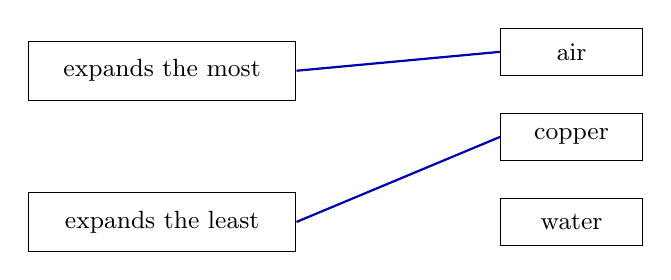
\begin{tikzpicture}[>=Stealth, font=\small, scale=0.8]
  \node[draw, minimum width=3.4cm, minimum height=0.75cm] (most) at (0,2.4) {expands the most};
  \node[draw, minimum width=3.4cm, minimum height=0.75cm] (least) at (0,0) {expands the least};
  \node[draw, minimum width=1.8cm, minimum height=0.6cm] (air) at (6.5,2.7) {air};
  \node[draw, minimum width=1.8cm, minimum height=0.6cm] (cu) at (6.5,1.35) {copper};
  \node[draw, minimum width=1.8cm, minimum height=0.6cm] (wat) at (6.5,0) {water};
  \draw[blue!70!black, thick] (most.east) -- (air.west);
  \draw[blue!70!black, thick] (least.east) -- (cu.west);
\end{tikzpicture}
\end{center}

For (b)(i)1, the \textbf{range} of a thermometer is the span of temperatures it is able to measure -- the \emph{difference between its lowest and highest readings}. For the thermometer in Fig.\,4.1 the scale runs from $0\,^{\circ}$C to $100\,^{\circ}$C, so its range is $0$--$100\,^{\circ}$C (a span of $100\,^{\circ}$C).

For (b)(i)2, \textbf{sensitivity} is how far the mercury thread moves for each degree of temperature change. A \emph{low} sensitivity means that for a given temperature rise the mercury expands only a little, so the degree marks lie very \textbf{close together} along the stem -- here the whole $100\,^{\circ}$C fits into a short scale. The practical consequence is that small temperature differences cannot be read.

For (b)(ii), to spread the same temperature change over a longer length of stem, increase the length of thread produced per degree. Since the thread length is $\Delta L = \Delta V / A$, where $\Delta V$ is the volume of liquid that expands and $A$ is the cross-sectional area of the bore, you can either increase $\Delta V$ or decrease $A$. So: use a \textbf{narrower bore} (thinner capillary tube), use a \textbf{larger bulb} so there is more liquid to expand, or choose a liquid with a larger expansivity (one that \textbf{expands more} per degree). Any one of these is enough.
\end{ansbox}

%=================================================================
\examq{5054/21/M/J/16}{5}{General Wave Properties \textperiodcentered\ Sound}{4}

\begin{mstab}{q5color}
 & sound: along or parallel (to transfer of energy or wave) \textbf{and} longitudinal & B1 \\ \cline{2-3}
\multirow{-2}{1.9cm}{5(a)} & water: perpendicular \textbf{and} transverse & B1 \\ \hline
5(b)(i) & $0.29$ -- $0.28$\,m & B1 \\ \hline
5(b)(ii) & time\,/\,period for one wave(length)\,/\,cycle constant\newline or each oscillation\,/\,cycle takes one second & B1 \\ \hline
\end{mstab}

\begin{ansbox}{q5color}
For (a), classify each wave by the direction in which the particles vibrate relative to the direction in which the energy travels.

\begin{itemize}[nosep,leftmargin=*]
\item \textbf{Sound}: the air is alternately compressed and rarefied, so each particle oscillates backwards and forwards \textbf{along (parallel to)} the direction in which the energy is transferred. A wave of this kind is \textbf{longitudinal}.
\item \textbf{Water} (ripples on the surface): each bit of the surface moves up and down, i.e.\ \textbf{perpendicular} to the direction in which the ripple travels. A wave of this kind is \textbf{transverse} -- the same as light, which is given in the table.
\end{itemize}

For (b)(i), the amplitude is the maximum displacement of the point from its undisturbed (mean) position, not the full height. The graph oscillates about a mean height of $1.00$\,m, and at $t = 0.25$\,s the point is at a crest, reaching about $1.28$--$1.29$\,m. Hence
\[ \text{amplitude} = 1.285 - 1.00 \approx 0.29\ \mathrm{m}. \]
(The wave is being damped, so the amplitude is quoted \emph{at that time}; anything in the range $0.28$--$0.29$\,m is accepted.)

For (b)(ii), frequency is $f = 1/T$, so a constant frequency means a constant period. Reading the graph, successive crests (or successive troughs, or successive zero-crossings in the same sense) are \textbf{equally spaced in time} -- one complete oscillation takes $1.0$\,s every time. Because the \textbf{time for one cycle does not change} as the wave passes, the frequency is constant. Note that this is true even though the amplitude is dying away: damping changes the amplitude, not the period.
\end{ansbox}

%=================================================================
\examq{5054/21/M/J/16}{6}{Light (Reflection/Refraction/Lenses)}{7}

\begin{mstab}{q6color}
 & angle of incidence & B1 \\ \cline{2-3}
\multirow{-2}{1.9cm}{6(a)} & smallest angle for light to be totally internally reflected\newline or largest angle (of incidence) for ray to be refracted\,/\,emerge\newline or when light emerges along surface\newline or when angle of refraction is $90^{\circ}$ & B1 \\ \hline
 & $n = 1/\sin C$ algebraic or numerical & C1 \\ \cline{2-3}
\multirow{-2}{1.9cm}{6(b)(i)} & 2.5 or 2.46 or $2.458(59)$ & A1 \\ \hline
 & left hand diagram ray refracts away from normal and emerges into air at bottom left surface & B1 \\ \cline{2-3}
 & right hand diagram reflected horizontal ray (by eye) & B1 \\ \cline{2-3}
\multirow{-3}{1.9cm}{6(b)(ii)} & right hand diagram rest of ray completely correct to emerge into air at top face without refraction (by eye) & B1 \\ \hline
\end{mstab}

\begin{ansbox}{q6color}
For (a), two ideas are needed. First, the critical angle is an \textbf{angle of incidence} -- measured from the normal, for a ray travelling \emph{inside} the optically denser medium (here the diamond) towards the boundary with the less dense one (air). Second, it is the particular value of that angle at which the behaviour changes: it is the \textbf{smallest angle of incidence at which the light is totally internally reflected}. Equivalent accepted statements: the largest angle of incidence for which the ray can still emerge (be refracted out); the angle for which the refracted ray grazes along the surface; the angle for which the angle of refraction is $90^{\circ}$.

For (b)(i), putting $r = 90^{\circ}$ into $n = \sin r / \sin i$ at the critical angle gives the standard result
\[ n = \frac{1}{\sin C} = \frac{1}{\sin 24^{\circ}} = \frac{1}{0.4067} = 2.4586 \approx 2.5. \]
A refractive index of about $2.5$ is very high (glass is about $1.5$), which is exactly why diamond has such a small critical angle and sparkles so strongly -- light entering it is trapped by total internal reflection at almost every face.

For (b)(ii), the single test to apply at each internal face is: \emph{compare the angle of incidence inside the diamond with $C = 24^{\circ}$}. If it is greater than $24^{\circ}$, the ray is totally internally reflected (angle of reflection $=$ angle of incidence, no light gets out). If it is less than $24^{\circ}$, the ray refracts out into the air, bending \textbf{away} from the normal as it does so (it is going from dense to less dense). If it hits a face along the normal, it passes straight through without bending.

\emph{Left-hand diamond.} Follow the ray to the bottom-left face. There its angle of incidence is \emph{less} than the critical angle, so it is not trapped: it \textbf{refracts away from the normal and emerges into the air at the bottom-left surface}.

\emph{Right-hand diamond.} At the first face the ray strikes at $45^{\circ}$, which is greater than $24^{\circ}$, so it is \textbf{totally internally reflected}; with the geometry of that face the reflected ray travels \textbf{horizontally} across the diamond. That horizontal ray then meets the \textbf{top face} along the normal (angle of incidence $0^{\circ}$), so it emerges there into the air \textbf{without being refracted} -- a straight line out, with no change of direction. The completed ray paths are shown below.
\begin{center}
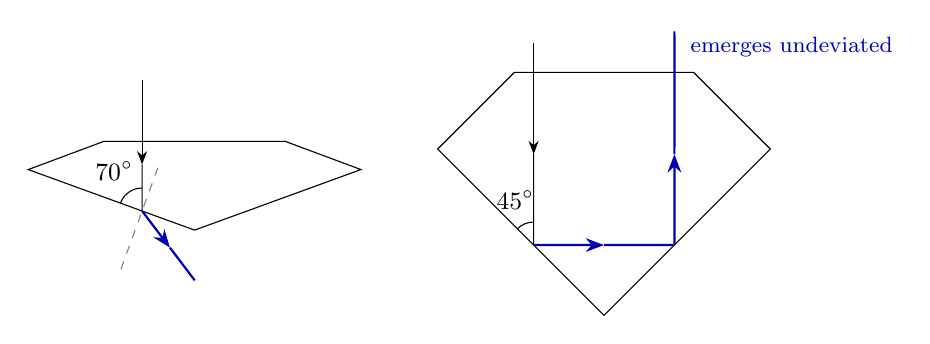
\begin{tikzpicture}[>=Stealth, font=\small, scale=0.65]
  % left-hand diamond (bottom-left face at 20 degrees to the horizontal)
  \draw (0,2.9) -- (1.475,3.45) -- (5.025,3.45) -- (6.5,2.9) -- (3.25,1.717) -- cycle;
  \coordinate (P) at (2.225,2.090);
  \draw[->] (2.225,4.65) -- (2.225,3.0);
  \draw (2.225,3.0) -- (P);
  \draw (P) ++(90:0.45) arc (90:160:0.45);
  \node at ($(P)+(125:0.95)$) {$70^{\circ}$};
  \draw[black!50, thin, dashed] ($(P)+(70:0.9)$) -- ($(P)+(250:1.3)$);
  \draw[blue!70!black, thick, ->] (P) -- ($(P)+(-52.8:0.9)$);
  \draw[blue!70!black, thick] ($(P)+(-52.8:0.9)$) -- ($(P)+(-52.8:1.7)$);
  % right-hand diamond (lower faces at 45 degrees)
  \draw (8,3.3) -- (9.5,4.8) -- (13.0,4.8) -- (14.5,3.3) -- (11.25,0.05) -- cycle;
  \coordinate (Q1) at (9.875,1.425);
  \coordinate (Q2) at (12.625,1.425);
  \coordinate (Q3) at (12.625,4.8);
  \draw[->] (9.875,5.375) -- (9.875,3.2);
  \draw (9.875,3.2) -- (Q1);
  \draw (Q1) ++(90:0.45) arc (90:135:0.45);
  \node at ($(Q1)+(112:0.95)$) {$45^{\circ}$};
  \draw[blue!70!black, thick, ->] (Q1) -- (11.25,1.425);
  \draw[blue!70!black, thick] (11.25,1.425) -- (Q2);
  \draw[blue!70!black, thick, ->] (Q2) -- (12.625,3.2);
  \draw[blue!70!black, thick] (12.625,3.2) -- (Q3) -- (12.625,5.6);
  \node[blue!70!black, right, font=\footnotesize] at (12.75,5.3) {emerges undeviated};
\end{tikzpicture}
\end{center}
\end{ansbox}

%=================================================================
\examq{5054/21/M/J/16}{7}{Electro Magnetism / Electromagnetic Induction \textperiodcentered\ Sound}{6}

\begin{mstab}{q7color}
7(a) & (current in coil) creates magnetic field\newline or current is at right angles to magnetic field (of permanent\,/\,cylindrical magnets) & C1 \\ \hline
 & into and out of magnet\newline or left and right\newline or backwards and forwards & B1 \\ \cline{2-3}
\multirow{-2}{1.9cm}{7(b)} & current is one way then reverses (so reverses force) & B1 \\ \hline
 & $(\lambda =)\ v/f$ numerically or algebraic in any form & C1 \\ \cline{2-3}
\multirow{-2}{1.9cm}{7(c)} & 0.64\,m & A1 \\ \hline
\end{mstab}

\begin{ansbox}{q7color}
For (a), this is the motor effect. The current in the coil \textbf{creates its own magnetic field}, and the coil sits in the field of the cylindrical permanent magnet, which runs radially across the turns -- so the \textbf{current is at right angles to the magnet's field}. The two fields interact (one side of the coil is reinforced, the other weakened), which produces a \textbf{force on the coil} along the axis of the magnet, in the direction given by Fleming's left-hand rule. The coil is attached to the paper cone, so the cone is pushed with it.

For (b), an alternating current \textbf{reverses direction} many times each second. Reversing the current reverses the direction of the current relative to the field, so by Fleming's left-hand rule the \textbf{force on the coil reverses} too. The cone is therefore pushed first one way and then the other -- it vibrates \textbf{backwards and forwards} (into and out of the magnet), once for each cycle of the current. These vibrations of the cone compress and rarefy the air in front of it, which is the sound wave; the cone vibrates at the frequency of the alternating current, so that is the frequency of the note produced.

For (c), use the wave equation $v = f\lambda$, rearranged:
\[ \lambda = \frac{v}{f} = \frac{320}{500} = 0.64\ \mathrm{m}. \]
Both quantities are already in SI units ($\mathrm{m\,/\,s}$ and Hz), so the wavelength comes out directly in metres.
\end{ansbox}

%=================================================================
\examq{5054/21/M/J/16}{8}{Electric Circuits \textperiodcentered\ Electrical Quantities}{4}

\begin{mstab}{q8color}
8(a)(i) & same\,/\,equal or $I_B = I_1 = I_2$ & B1 \\ \hline
8(a)(ii) & (p.d.\ of) battery is sum of (p.d.\ across) fixed resistor and (p.d.\ across) the variable resistor\newline or $V_B = V_1 + V_2$ & B1 \\ \hline
 & $(I =)\ V/R$ numerical or algebraic in any form & C1 \\ \cline{2-3}
\multirow{-2}{1.9cm}{8(b)} & $0.006(0)$\,A & A1 \\ \hline
\end{mstab}

\begin{ansbox}{q8color}
For (a)(i), the battery, the fixed resistor and the variable resistor form a \textbf{single loop} -- there is nowhere for the charge to branch off. Charge is conserved, so the same current passes through every component in turn:
\[ I_B = I_1 = I_2 \quad \text{(all equal)}. \]

For (a)(ii), energy is conserved around the loop: the energy each coulomb gains in the battery is exactly the energy it loses in the two resistors. So the p.d.\ across the battery equals the \textbf{sum} of the p.d.s across the two resistors:
\[ V_B = V_1 + V_2. \]

For (b), because the two resistors are in series their resistances simply add:
\[ R_{\text{total}} = 1000 + 500 = 1500\ \Omega. \]
The whole $9.0$\,V of the battery is across this combination, so from $V = IR$,
\[ I = \frac{V}{R} = \frac{9.0}{1500} = 0.0060\ \mathrm{A}\ (6.0\ \mathrm{mA}). \]
By (a)(i) this \emph{is} the current in R, since the current is the same everywhere in a series circuit. (As a check, the p.d.s are $0.0060 \times 1000 = 6.0$\,V and $0.0060 \times 500 = 3.0$\,V, which add to $9.0$\,V as (a)(ii) requires.)
\end{ansbox}

%=================================================================
\examq{5054/21/M/J/16}{9}{Uses of Oscilloscope \textperiodcentered\ Electric Circuits}{4}

\begin{mstab}{q9color}
 & 2 squares & C1 \\ \cline{2-3}
\multirow{-2}{1.9cm}{9\,E\,(a)} & 10\,V & A1 \\ \hline
 & measure\,/\,find horizontal distance\,/\,number of divisions (between points) & C1 \\ \cline{2-3}
\multirow{-2}{1.9cm}{9\,E\,(b)} & distance $\times$ no (m)s\,/\,division & A1 \\ \hline
9\,OR\,(a) & transistor & B1 \\ \hline
 & (in dark) resistance of LDR large\,/\,increases & B1 \\ \cline{2-3}
 & large voltage across base (and emitter) & B1 \\ \cline{2-3}
\multirow{-3}{1.9cm}{9\,OR\,(b)} & switches transistor on\newline or current in collector increases & B1 \\ \hline
\end{mstab}

\begin{ansbox}{q9color}
Only \emph{one} of the two alternatives is answered in the examination; both are worked here.

\medskip
\textbf{EITHER -- the cathode-ray oscilloscope.}

For (a), the Y-gain control sets how many volts correspond to one vertical division of the grid. In Fig.\,9.1 the Y-gain is set to $5$\,V\,/\,division. The \emph{maximum} (peak) voltage is the vertical distance from the centre line of the trace up to a crest, which is \textbf{2 squares} (divisions). Hence
\[ V_{\max} = 2 \times 5 = 10\ \mathrm{V}. \]
Read the peak from the \emph{centre} line, not from trough to crest -- trough to crest would be 4 divisions and would give the peak-to-peak voltage, $20$\,V.

For (b), the time-base control plays the same role horizontally: it sets how many milliseconds correspond to one horizontal division. So to find the time between any two points on the trace, \textbf{count the horizontal distance between them in divisions} (estimating fractions of a division by eye), read the \textbf{time-base setting} in ms\,/\,division, and \textbf{multiply}:
\[ \text{time} = (\text{number of divisions}) \times (\text{ms per division}). \]
Divide by $1000$ if the answer is wanted in seconds.

\medskip
\textbf{OR -- the automatic night light.}

For (a), component A is a \textbf{transistor}. It is being used as an electrically operated switch: a small current into its base allows a much larger current to flow through the lamp in its collector circuit.

For (b), the LDR and the other resistor form a potential divider across the supply, and the voltage across one of them is applied to the base of the transistor. A light-dependent resistor has a high resistance in the dark and a low resistance in bright light. So when it gets dark, the \textbf{resistance of the LDR increases} (becomes large). That changes the way the supply voltage is shared, so a \textbf{larger voltage now appears across the base--emitter junction} of the transistor. Once that base voltage rises above about $0.6$\,V the transistor is \textbf{switched on}: a base current flows, a much larger \textbf{collector current flows} through the lamp, and the lamp lights. When daylight returns the LDR's resistance falls, the base voltage drops below $0.6$\,V, the transistor switches off and the lamp goes out.
\end{ansbox}

%=================================================================
\examq{5054/21/M/J/16}{10}{Thermal Properties \& Temperature \textperiodcentered\ Kinetic Model of Matter \textperiodcentered\ Transfer of Thermal Energy}{15}

\begin{mstab}{q10color}
 & temperature & B1 \\ \cline{2-3}
\multirow{-2}{1.9cm}{10(a)(i)} & when solid turns to liquid & B1 \\ \hline
 & molecules escape (surface) & C1 \\ \cline{2-3}
 & fastest molecules\,/\,most energetic molecules escape\,/\,break bonds & A1 \\ \cline{2-3}
\multirow{-3}{1.9cm}{10(a)(ii)} & leaving behind slower molecules\,/\,colder molecules\newline or temperature falls & B1 \\ \hline
10(b)(i) & at the surface\,/\,top of liquid & B1 \\ \hline
 & less heat\,/\,energy enters (liquid nitrogen)\,/\,transfers\newline or less nitrogen evaporates\,/\,boils & B1 \\ \cline{2-3}
 & reduces\,/\,stops conduction and convection & B1 \\ \cline{2-3}
\multirow{-3}{1.9cm}{10(b)(ii)} & explanation of no conduction or convection, e.g.\ no molecules\,/\,no medium & B1 \\ \hline
10(c)(i) & nitrogen gas or nitrogen vapour & B1 \\ \hline
 & $(Q =)\ mc\Delta T$ numerical or algebraic & C1 \\ \cline{2-3}
 & $216\ (^{\circ}\mathrm{C})$ seen & C1 \\ \cline{2-3}
\multirow{-3}{1.9cm}{10(c)(ii)1} & 4200\,J & A1 \\ \hline
 & $(m =)\ Q/L$ numerical or algebraic & C1 \\ \cline{2-3}
\multirow{-2}{1.9cm}{10(c)(ii)2} & 21\,g & A1 \\ \hline
\end{mstab}

\begin{ansbox}{q10color}
For (a)(i), two ideas earn the two marks: the melting point is a \textbf{temperature}, and it is the temperature \textbf{at which a solid turns into a liquid}. (At that temperature the energy supplied goes into breaking the bonds that hold the molecules in their fixed lattice positions, so the temperature stays constant while the solid melts.)

For (a)(ii), evaporation happens at the surface and is a \emph{selective} process. The molecules in a liquid do not all have the same speed: there is a spread of molecular energies. Only the \textbf{fastest, most energetic molecules} near the surface have enough energy to \textbf{break the bonds} holding them in the liquid and \textbf{escape} through the surface into the space above. Because it is the most energetic molecules that leave, the ones \textbf{left behind are the slower, less energetic} ones, so the average kinetic energy of the remaining liquid falls -- and since temperature is a measure of average molecular kinetic energy, \textbf{the temperature of the liquid falls}. That is why evaporation produces cooling.

For (b)(i), evaporation requires molecules to escape through a free surface, so it occurs \textbf{at the surface (top) of the liquid nitrogen}, where the liquid meets the space above it.

For (b)(ii), state the advantage, then explain it. The advantage: \textbf{less thermal energy enters the liquid nitrogen} from the warm surroundings, so \textbf{less nitrogen boils away} and it can be stored for much longer. The explanation: energy can only be conducted or convected if there are molecules to carry it. Conduction needs a material medium whose particles can pass vibrations (or free electrons) from one to the next, and convection needs a fluid that can physically circulate. A \textbf{vacuum contains no molecules -- no medium at all}, so \textbf{neither conduction nor convection can cross the gap} between the two glass walls. (Only radiation can cross a vacuum, which is why the walls of a real vacuum flask are also silvered.)

For (c)(i), the liquid is boiling, so the bubbles forming inside it are bubbles of the liquid's own vapour: \textbf{nitrogen gas (nitrogen vapour)}. They are not air -- air would have been expelled long before, and at $-196\,^{\circ}$C most of it would be liquid anyway.

For (c)(ii)1, the metal cools from $20\,^{\circ}$C to $-196\,^{\circ}$C, so the temperature \emph{change} is
\[ \Delta T = 20 - (-196) = 216\ ^{\circ}\mathrm{C}. \]
Getting this subtraction right is worth a mark on its own. Then, with $m = 50$\,g and $c = 0.39\ \mathrm{J/(g\,^{\circ}C)}$ -- note that $c$ is given per \emph{gram}, so there is no need to convert to kilograms:
\[ Q = mc\Delta T = 50 \times 0.39 \times 216 = 4212\ \mathrm{J} \approx 4200\ \mathrm{J}. \]

For (c)(ii)2, all of that energy is given to the liquid nitrogen, which is already at its boiling point, so it is used entirely to boil nitrogen away (no further temperature rise is possible). Using $Q = mL$ with $L = 200$\,J\,/\,g:
\[ m = \frac{Q}{L} = \frac{4212}{200} = 21.06\ \mathrm{g} \approx 21\ \mathrm{g}. \]
Use the unrounded $4212$\,J here; the rounded $4200$\,J gives $21.0$\,g, the same answer to two significant figures.
\end{ansbox}

%=================================================================
\examq{5054/21/M/J/16}{11}{Electro Magnetism / Electromagnetic Induction \textperiodcentered\ Electrical Quantities}{15}

\begin{mstab}{q1color}
 & diagram showing coil of wire and either\newline $\bullet$ magnet or\newline $\bullet$ another coil and supply (dc and switch or ac) & B1 \\ \cline{2-3}
 & coil of wire connected to an ammeter or voltmeter or cro or other method of detection, e.g.\ lamp & B1 \\ \cline{2-3}
\multirow{-3}{1.9cm}{11(a)(i)} & magnet or coil moved\newline or change in current mentioned if another coil used & B1 \\ \hline
11(a)(ii) & ANY 2 from\newline $\bullet$ move magnet (or coil) faster\newline $\bullet$ larger current in primary (if transformer drawn)\newline $\bullet$ more turns in coil\newline $\bullet$ stronger magnet (if magnet drawn)\newline $\bullet$ soft iron core & B2 \\ \hline
 & direction of induced current\,/\,induced emf & B1 \\ \cline{2-3}
\multirow{-2}{1.9cm}{11(a)(iii)1} & opposes the change (that produces it) & B1 \\ \hline
 & (magnetic) flux\,/\,field\,/\,poles in coil caused by movement\,/\,(induced) current in coil & B1 \\ \cline{2-3}
\multirow{-2}{1.9cm}{11(a)(iii)2} & statement of how opposition occurs, e.g.\ repulsion as magnet moves in; N pole created (by induction) at end of coil as N pole approaches & B1 \\ \hline
 & $(I =)\ P/V$ numerical or algebraic & C1 \\ \cline{2-3}
\multirow{-2}{1.9cm}{11(b)(i)1} & $15(.15)$\,A & A1 \\ \hline
 & $(E =)\ Pt$ or $VIt$ or $500(000) \times 60 \times 60$ & C1 \\ \cline{2-3}
\multirow{-2}{1.9cm}{11(b)(i)2} & $1.8 \times 10^{9}$\,J or 500\,kWh & A1 \\ \hline
 & low current & B1 \\ \cline{2-3}
\multirow{-2}{1.9cm}{11(b)(ii)} & $P = I^2R$ or $E = I^2Rt$ explained & B1 \\ \hline
\end{mstab}

\begin{ansbox}{q1color}
For (a)(i), the simplest demonstration needs three things, and the mark scheme awards one mark for each. Sketch a \textbf{coil of wire} (a solenoid of many turns). Connect its two ends to a \textbf{sensitive centre-zero ammeter} (galvanometer) -- or a voltmeter, c.r.o.\ or even a lamp -- so that an induced current can be detected, and label it. Then show a bar \textbf{magnet being moved} into (or out of) the coil, with an arrow and a label such as ``magnet pushed in''. The demonstration: as the magnet moves, the needle deflects; when the magnet is held still inside the coil, the needle returns to zero; when the magnet is pulled out, the needle deflects the \emph{other} way. (The alternative arrangement, worth the same marks, is a second coil wound alongside and connected to a supply, with the current in it switched on and off or supplied as a.c.) A suitable sketch is shown below.
\begin{center}
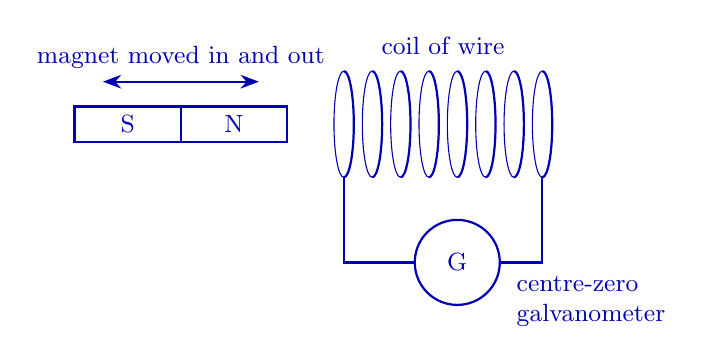
\begin{tikzpicture}[>=Stealth, font=\small, scale=0.9]
  % coil of wire (solenoid)
  \foreach \x in {0,0.4,...,2.81} {
    \draw[blue!70!black, thin] (\x,1.5) arc (90:270:0.14 and 0.75);
    \draw[blue!70!black, thick] (\x,0) arc (-90:90:0.14 and 0.75);
  }
  \draw[blue!70!black, thick] (0,0) -- (0,-1.2) -- (1.0,-1.2);
  \draw[blue!70!black, thick] (2.8,0) -- (2.8,-1.2) -- (2.2,-1.2);
  % centre-zero galvanometer
  \draw[blue!70!black, thick, fill=white] (1.6,-1.2) circle (0.6);
  \node[blue!70!black] at (1.6,-1.2) {G};
  % bar magnet being pushed in
  \draw[blue!70!black, thick] (-3.8,0.5) rectangle (-0.8,1.0);
  \draw[blue!70!black, thick] (-2.3,0.5) -- (-2.3,1.0);
  \node[blue!70!black] at (-3.05,0.75) {S};
  \node[blue!70!black] at (-1.55,0.75) {N};
  \draw[blue!70!black, thick, <->] (-3.4,1.35) -- (-1.2,1.35);
  \node[blue!70!black, above] at (-2.3,1.4) {magnet moved in and out};
  \node[blue!70!black, above] at (1.4,1.6) {coil of wire};
  \node[blue!70!black, right, align=left] at (2.3,-1.75) {centre-zero\\galvanometer};
\end{tikzpicture}
\end{center}

For (a)(ii), the induced e.m.f.\ is proportional to the \emph{rate of change of flux linkage}, so anything that increases the flux or the speed of its change increases the induced current. Any \textbf{two} of: \textbf{move the magnet (or coil) faster}; use \textbf{more turns} on the coil; use a \textbf{stronger magnet}; insert a \textbf{soft-iron core}; or, if the two-coil version was drawn, use a \textbf{larger current in the primary}.

For (a)(iii)1, Lenz's law states that the \textbf{direction of the induced current (or induced e.m.f.)} is always such as to \textbf{oppose the change that produced it}. Both halves are needed -- naming what the law is about, and the opposition.

For (a)(iii)2, apply it to the demonstration. The induced current flowing round the coil makes the coil itself into an electromagnet, so it has its \textbf{own magnetic field and poles}. The direction of that current is such that the end of the coil nearest the approaching magnet becomes the \emph{same} pole as the magnet's leading pole -- so if a \textbf{N pole is pushed in, a N pole is induced at that end of the coil}, and the two \textbf{repel}, opposing the magnet's motion inwards. Pull the magnet out again and the current reverses, a S pole appears at that end, and the coil now \emph{attracts} the magnet -- again opposing the motion. (This is energy conservation at work: you must do work against that opposing force, and that work is the source of the electrical energy generated.)

For (b)(i)1, from $P = VI$, keeping the units consistent ($500\,\mathrm{kW} = 5.00 \times 10^5$\,W, $33\,\mathrm{kV} = 3.3 \times 10^4$\,V):
\[ I = \frac{P}{V} = \frac{5.00 \times 10^{5}}{3.3 \times 10^{4}} = 15.15 \approx 15\ \mathrm{A}. \]

For (b)(i)2, energy is power $\times$ time, with one hour $= 60 \times 60 = 3600$\,s:
\[ E = Pt = 5.00 \times 10^{5} \times 3600 = 1.8 \times 10^{9}\ \mathrm{J}. \]
In commercial units this is $500\,\mathrm{kW} \times 1\,\mathrm{h} = 500$\,kW\,h, which is the same energy.

For (b)(ii), for a fixed power delivered, $P = VI$ means that raising the transmission voltage makes the \textbf{current low} -- here only about $15$\,A for half a megawatt. The energy wasted heating the transmission lines depends on the current through their resistance $R$:
\[ P_{\text{lost}} = I^2R \qquad (E_{\text{lost}} = I^2Rt), \]
which goes as the \emph{square} of the current. So reducing the current by a factor of ten cuts the heating loss by a factor of a hundred. Transmitting at $33$\,kV rather than at a few hundred volts therefore wastes far less of the generated energy in the cables.
\end{ansbox}

%=================================================================
\examq{5054/21/M/J/16}{12}{Motion or Kinematics \textperiodcentered\ Forces or Dynamics \textperiodcentered\ Work Energy and Power \textperiodcentered\ Pressure}{15}

\begin{mstab}{q2color}
 & kinetic energy at start & B1 \\ \cline{2-3}
\multirow{-2}{1.9cm}{12(a)} & thermal energy\,/\,heat energy\,/\,internal energy at end & B1 \\ \hline
12(b)(i) & $0.4(0)$\,s & B1 \\ \hline
 & $(d =)\ s \times t$ numerical or algebraic & C1 \\ \cline{2-3}
\multirow{-2}{1.9cm}{12(b)(ii)} & 2.8\,m & A1 \\ \hline
12(b)(iii) & area under graph (between 0.4 and 2.4\,s)\newline or time (difference) $\times$ average speed\newline or $\frac{1}{2} \times$ time (difference) $\times$ initial speed & B1 \\ \hline
 & horizontal line from $(0,5)$ to $(0.4,5)$ & B1 \\ \cline{2-3}
\multirow{-2}{1.9cm}{12(b)(iv)} & line showing braking with same gradient as original line & B1 \\ \hline
 & less friction & B1 \\ \cline{2-3}
 & less deceleration or graph less steep\newline or less force backwards\,/\,less force opposing motion\newline or same KE lost\,/\,work done by friction & B1 \\ \cline{2-3}
\multirow{-3}{1.9cm}{12(b)(v)} & longer time to stop\newline or larger area under (speed-time) graph\newline or work $=$ force $\times$ distance applied correctly & B1 \\ \hline
 & $(F =)\ P \times A$ numerical or algebraic & C1 \\ \cline{2-3}
\multirow{-2}{1.9cm}{12(c)(i)} & 60\,N & A1 \\ \hline
 & same pressure & B1 \\ \cline{2-3}
\multirow{-2}{1.9cm}{12(c)(ii)} & larger area (of S\,/\,brake pads) & B1 \\ \hline
\end{mstab}

\begin{ansbox}{q2color}
For (a), name the energy at each end of the process. At the start the cyclist is moving, so the energy is \textbf{kinetic energy}. The brake pads rub against the spinning disc, and friction does work against the motion; by the time the cycle has stopped all of that kinetic energy has been transferred to \textbf{thermal (internal) energy} in the pads, the disc and the surrounding air -- which is why disc brakes get hot.

For (b)(i), during the reaction time the cyclist has not yet touched the brakes, so the speed is unchanged -- that is the \emph{horizontal} part of the graph at the start. It lasts until the line begins to fall, at
\[ \text{reaction time} = 0.4\ \mathrm{s}. \]

For (b)(ii), during those $0.4$\,s the speed is constant at $7.0$\,m\,/\,s (read from the flat part of Fig.\,12.2), so
\[ \text{thinking distance} = \text{speed} \times \text{time} = 7.0 \times 0.4 = 2.8\ \mathrm{m}. \]
(Equivalently it is the area of the rectangle under the flat section of the graph.)

For (b)(iii), on any speed--time graph the distance travelled is the \textbf{area under the graph}. The braking distance is therefore the area under the \emph{sloping} part, between $t = 0.4$\,s and $t = 2.4$\,s. That region is a triangle, so it can also be worked out as $\frac{1}{2} \times \text{time} \times \text{initial speed}$, or as (time difference) $\times$ (average speed):
\[ \tfrac{1}{2} \times 2.0 \times 7.0 = 7.0\ \mathrm{m}. \]

For (b)(iv), two features must be right. First, the reaction time is unchanged, so start with a \textbf{horizontal line from $(0, 5.0)$ to $(0.4, 5.0)$} -- flat, at the new initial speed of $5.0$\,m\,/\,s. Second, the deceleration is unchanged, so the braking part must be a straight line with the \textbf{same gradient as the original}. The original line falls from $7.0$\,m\,/\,s to zero in $2.0$\,s, a gradient of $-3.5\ \mathrm{m/s^2}$; starting from $5.0$\,m\,/\,s at the same gradient takes $5.0/3.5 = 1.4$\,s, so the new line runs from $(0.4, 5.0)$ down to the time axis at about $t = 1.8$\,s. The new graph is parallel to the old one, just lower and shorter. The new graph is shown below.
\begin{center}
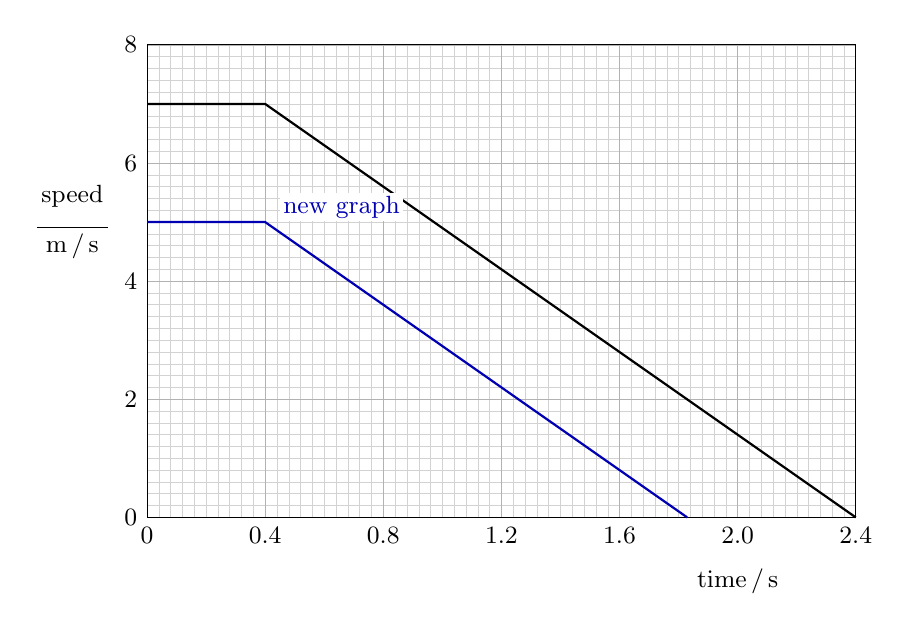
\begin{tikzpicture}[>=Stealth, font=\small, xscale=3.75, yscale=0.75]
  \fill[white] (0,0) rectangle (2.4,8);
  \foreach \x in {0.04,0.08,...,2.39} \draw[gray!35, very thin] (\x,0) -- (\x,8);
  \foreach \y in {0.2,0.4,...,7.9} \draw[gray!35, very thin] (0,\y) -- (2.4,\y);
  \foreach \x in {0,0.4,...,2.41} \draw[gray!60, very thin] (\x,0) -- (\x,8);
  \foreach \y in {0,2,...,8} \draw[gray!60, very thin] (0,\y) -- (2.4,\y);
  \draw (0,0) rectangle (2.4,8);
  \foreach \x/\l in {0/0,0.4/0.4,0.8/0.8,1.2/1.2,1.6/1.6,2.0/2.0,2.4/2.4} \node[below] at (\x,0) {\l};
  \foreach \y in {0,2,4,6,8} \node[left] at (0,\y) {\y};
  \node[below] at (2.0,-0.7) {time\,/\,s};
  \node[left, align=center] at (-0.1,5) {speed\\[-2pt]\rule{0.9cm}{0.4pt}\\[-2pt]m\,/\,s};
  % original graph (given)
  \draw[thick] (0,7) -- (0.4,7) -- (2.4,0);
  % new graph (answer)
  \draw[blue!70!black, thick] (0,5) -- (0.4,5) -- (1.829,0);
  \node[blue!70!black, fill=white, inner sep=1pt, right] at (0.45,5.25) {new graph};
\end{tikzpicture}
\end{center}

For (b)(v), three linked steps earn the three marks. On a wet road there is \textbf{less friction} between the tyres and the road (and between the pads and a wet disc), so the maximum \textbf{backward force opposing the motion is smaller}. By $F = ma$, a smaller force means a smaller \textbf{deceleration}, so the braking line on the graph is \textbf{less steep}. The cyclist starts with the same kinetic energy and must still lose all of it, so with a smaller braking force the cycle takes a \textbf{longer time to stop} and the area under the speed--time graph (the distance) is \textbf{larger}. Put energetically: work done $= $ force $\times$ distance, so if the same kinetic energy must be removed by a smaller force, the distance has to be greater.

For (c)(i), rearranging $p = F/A$:
\[ F = p \times A = 1.2 \times 10^{6} \times 5.0 \times 10^{-5} = 60\ \mathrm{N}. \]
Both quantities are in SI units (Pa and $\mathrm{m^2}$), so the force comes out in newtons directly.

For (c)(ii), the oil is a liquid and is practically incompressible, so the pressure increase produced at piston R is transmitted undiminished throughout the oil: the \textbf{same pressure} acts on piston S. But force $= $ pressure $\times$ area, so with the same pressure a \textbf{larger piston (and brake-pad) area} gives a \textbf{larger force}. That is the point of a hydraulic system -- it multiplies the force by the ratio of the piston areas.
\end{ansbox}

\end{document}
